\documentclass[letterpaper,10pt]{article}

\setlength{\evensidemargin}{-0.0in}
\setlength{\oddsidemargin}{-0.0in}
\setlength{\textwidth}{6.4in}

\usepackage[utf8]{inputenc}
\usepackage{amsmath,calligra,mathrsfs}
\usepackage{amssymb}
\usepackage{enumerate}
\usepackage{mathpazo}
\usepackage{relsize}
\usepackage{mathtools}
\usepackage{verbatim}

\usepackage{hyperref}
\hypersetup{
    colorlinks=true,
    linkcolor=blue,
    filecolor=magenta,      
    urlcolor=blue,
}

\usepackage{tikz}
\usetikzlibrary{matrix,arrows}

\usepackage{fancyhdr}
\pagestyle{fancy}
\lhead{Stability on surfaces}
\rhead{Tuomas Tajakka}
%\cfoot{}
\rfoot{}
\renewcommand{\headrulewidth}{0.4pt}

\usepackage{amsthm}
\newtheorem{thm}{Theorem}[section]
\newtheorem{lem}[thm]{Lemma}
\newtheorem{prop}[thm]{Proposition}
\newtheorem{cor}[thm]{Corollary}
\newtheorem{expl}[thm]{Example}
\newtheorem{defn}[thm]{Definition}
\newtheorem{rmk}[thm]{Remark}
\newtheorem{exer}[thm]{Exercise}

\title{Stability on Surfaces}
\author{Tuomas Tajakka}
\date{}

\usepackage{commands}

\begin{document}

\begin{center}
    \LARGE{Stability on Surfaces}
\end{center}

\section{Definitions of slope}
Let $X$ be a projective variety of dimension $n$ (over $k = \overline{k}$ maybe), with a very ample line bundle $\Oh_X(1)$.

If $E$ is a coherent sheaf on $X$ with $d$-dimensional support, in Huybrechts-Lehn (HL) it is proved that the the Hilbert polynomial $P(E, m) = \chi(X, E(m))$ can be written uniquely as
\[ P(E, m) = \sum_{i=0}^d \al_i(E) \frac{m^i}{i!} \]
for integers $\al_i(E), i = 0, \ldots, d$, and $\al_d(E) > 0$.  

\subsection{Rank}
If $E$ is $n$-dimensional, the rank of $E$ is defined in HL as
\[ \rk(E) = \frac{\al_n(E)}{\al_n(\Oh_X)}. \]
Let's check that if $X$ is integral, then this definition agrees with the usual one, $\rk(E) = \dim_{\Oh_{X,\eta}}(E_\eta)$, where $\eta \in X$ is the generic point. Choose $N \in \Z$ such that the stalk $E(N)_\eta$ has basis the images of $r$ global sections. This gives a map
\[ \Oh_X(-N)^{\oplus r} \to E, \]
that is generically an isomorphism. This means that the Hilbert polynomials of $E$ and $\Oh_X(-N)^{\oplus r}$ have the same leading term, that is,
\[ \al_n(E) = \al_n(\Oh_X(-N)^{\oplus r}) = r \al_n(\Oh_X(-N)). \]
Now
\[ P(\Oh_X(-N), m) = P(\Oh_X, m - N) = \al_n(\Oh_X) \frac{(m-N)^n}{n!} + \mathrm{l.o.t.}. \]
The coefficient of the leading term is still $\frac{\al_n(\Oh_X)}{n!}$, which means that $\al_n(\Oh_X(-N)) = \al_n(\Oh_X)$. The result follows.

\subsection{Slope}


\subsection{HN-filtration for $\mu$-stability}
Let $E$ be a coherent sheaf on $X$. The torsion subsheaf $E_{tors} \subs E$ is supported in positive codimension, and the quotient $F = E/E_{tors}$ is torsion free. By HL, Theorem 1.3.4, $F$ has a unique Harder-Narasimhan filtration
\[ 0 = F_0 \subset F_1 \subset \cdots \subset F_r = F. \]
If $\pi: E \to F$ is the quotient map, setting $E_i = \pi^{-1}(F_i)$ gives a filtration
\[ 0 \subset E_0 = E_{tors} \subset E_1 \subset \cdots \subset E_r = E \]
of $E$, such that each quotient is either torsion or Gieseker semistable. 

\begin{lem}
    If $0 \to E' \to E \to E'' \to 0$ is an exact sequence of torsion-free sheaves such that $\mu(E'), \mu(E'') \le \be$, then also $\mu(E) \le \be$.
\end{lem}
\begin{proof}
    The condition is equivalent to $\al_1(E') \le \be \al_2(E'), \; \al_1(E'') \le \be \al_2(E'')$. Now
    \[ \al_1(E) = \al_1(E') + \al_1(E'') \le \be \al_2(E') + \be \al_2(E'') = \be \al_2(E), \]
    which is equivalent to the claim.
\end{proof}

It follows by induction from this lemma that if a torsion-free sheaf $F$ has a filtration
\[ 0 = F_0 \subset F_1 \subset \cdots \subset F_r = F \]
such that $\mu(F_i/F_{i-1}) \le \be$ for all $i$, then $\mu(F) \le \be$.

\begin{lem}
    Let $\be \in \Q$. If $E$ is a torsion-free sheaf with HN-filtration
    \[ 0 = F_0 \subset F_1 \subset \cdots \subset F_r = F \]
    with respect to Gieseker stability such that $\mu(F_i/F_{i-1}) = \be$ for all $i$, then $F$ is $\mu$-semistable.
\end{lem}
\begin{proof}
    If $G \subs F$ is a nonzero subsheaf, then $G$ has a filtration by the subsheaves $G_i = G \cap F_i$. Now $G_i/G_{i-1} \subs F_i/F_{i-1}$, so since $F_i/F_{i-1}$ is $\mu$-semistable, we have
    \[ \mu(G_i/G_{i-1}) \le \mu(F_i/F_{i-1}) = \be. \]
    The previous lemma (and it's generalization) finishes the proof.
\end{proof}

Now starting with the above filtration
\[ 0 \subset E_0 = E_{tors} \subset E_1 \subset \cdots \subset E_r = E, \]
if we drop the terms where the slopes of the quotients don't change, we obtain a filtration that starts with the torsion subsheaf, and is followed by torsion-free subsheaves such that the quotients are $\mu$-semistable with strictly decreasing slopes.


\section{Tilting of hearts}
If $\sA \subs \sD$ is the heart of a bounded t-structure in a triangulated category, a torsion pair on $\sA$ is a pair of two full additive subcategories $(\sF, \sT)$ of $\sA$, such that for any $F \in \sF, T \in \sT$, we have $\Hom_\sA(T, F) = 0$, and any object $E \in \sA$ fits in a short exact sequence
\[ 0 \to T \to E \to F \to 0 \]
in $\sA$ with $T \in \sT, F \in \sF$.

If $(\sF, \sT)$ is a torsion pair on $\sA$, we define a full additive subcategory $\sA^\#$ whose objects $E$ are those objects in $\sD$ that fit in an exact triangle
\[ F[1] \to E \to T \]
with $F \in \sF, T \in \sT$. It is proven in [Macri-Schmidt] that $\sA^\#$ satisfies the Hom-requirement of a heart of a bounded t-structure. We prove here the existence of HN-filtrations.

Let $E \in \sD$ with HN-filtration with respect to $\sA$
\begin{center}
        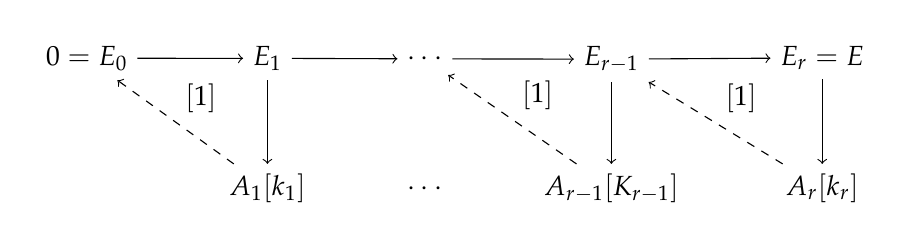
\begin{tikzpicture}
        \matrix (m) [matrix of math nodes, row sep=3em, column sep=3em]
        { 0 = E_0 & E_1 & \cdots & E_{r-1} & E_r = E \\
        & A_1[k_1] & \cdots & A_{r-1}[K_{r-1}] & A_r[k_r] \\};
        \path[->] 
        (m-1-1) edge node[auto] {$ $} (m-1-2)
        (m-1-2) edge node[auto] {$ $} (m-1-3)
        (m-1-3) edge node[auto] {$ $} (m-1-4)
        (m-1-4) edge node[auto] {$ $} (m-1-5)
        (m-1-2) edge node[auto] {$ $} (m-2-2)
        (m-1-4) edge node[auto] {$ $} (m-2-4)
        (m-1-5) edge node[auto] {$ $} (m-2-5)
        ;
        \path[dashed,->]
        (m-2-5) edge node[auto,swap] {$ [1] $} (m-1-4)
        (m-2-2) edge node[auto,swap] {$ [1] $} (m-1-1)
        (m-2-4) edge node[auto,swap] {$ [1] $} (m-1-3)
        ;        
        \end{tikzpicture}
\end{center}
with $A_1, \ldots, A_m \in \sA$, and $k_1 > k_2 > \cdots > k_m$. For each $i$, let 
\[ 0 \to T_i \to A_i \to F_i \to 0 \]
be the unique short exact sequence in $\sA$ with $T_i \in \sT, F_i \in \sF$.

Let $l$ be the largest index such that $k_i - k_{i+1} = 1$ for all $i > l$. For each $l \le i \le r-1$, let $E_i^\#$ be the unique object such that the triangle
\[ E_i^\# \to E_{i+1} \to F_{i+1}[k_{i+1}] \]
is exact, where the second map is the composition 
\[ E_{i+1} \to A_{i+1}[k_{i+1}] \to F_{i+1}[k_{i+1}]. \]
By the Octahedral axiom, we have exact triangles
\[ E_i \to E_i^\# \to T_{i+1}[k_{i+1}], \]
and
\[ F_{i-1}[k_{i-1}] \to A_i^\# \to T_i[k_i], \]
where $A_i^\#$ is the cone of the composition
\[ E_{i-1}^\# \to E_i \to E_i^\#. \]
Thus, we have a sequence of maps
\[ E_l^\# \to E_{l+1}^\# \to \cdots \to E_{r-1}^\# \to E_r^\# \to E_r \]
with cones $A_i^\# \in \sA^\#[k_i]$. Moreover, the cone of the map $E_l \to E_l^\#$ is $T_{l+1}[k_{l+1}] \in \sA^\#[k_{l+1}]$. By induction on the length of the filtration, $E_l$ has an HN-filtration with respect to $\sA^\#$ with last factor in $\sA^\#[k_l-1]$. Concatenating this filtration with the newly produced one by the map $E_l \to E_l^\#$ creates the HN-filtration for $E$.


\section{Gieseker vs. twisted Gieseker stability}

(This is discussed in \emph{Mumford-Thaddeus Principle on the Moduli Space
of Vector Bundles on an Algebraic Surface} by Matsuki and Wentworth)

Let $H \in N^1(X)$ be an ample real divisor class, and let $B \in N^1(X)$ be any divisor class. We define the {\bf $B$-twisted Chern character} by
\[ \ch^B = \ch \cdot e^{-B} = C_0 + C_1 - C_0 B + C_2 - B \cdot C_1 + \frac{1}{2} C_0 B^2. \]
Since the Chern character is a ring homomorhism, and $\ch(L) = e^{c_1(L)}$ for a line bundle $L$, we have
\[ \ch^B(E) = \ch(E) e^{-B} = \ch(E) \ch(-B) = \ch(E(-B)). \]
The {\bf $B$-twisted Hilbert polynomial} of $E \in \Coh(X)$ is defined by
\[ P(E, B, t) = \int_X \ch^B(E) e^{t H} \td(X) = a_2(E, B) t^2 + a_1(E, B) t + a_0(E, B), \]
and the corresponding reduced polynomial by
\[ p(E, B, t) = \frac{P(E, B, t)}{a_2(E, B)}. \]
Notice that this differs from HL by a factor of $\frac{1}{2}$. Notice also that if $B$ is an integral class, i.e. represented by a line bundle, 
\[ P(E, B, t) = P(E(-B), t). \]

We say $E \in \Coh(X)$ is {\bf $B$-twisted Gieseker (semi)stable} if for any proper non-trivial subsheaf $F \subs E$,
\[ p(F, B, t) < (\leq) p(E, B, t). \]

Let's write out explicitly the coefficients $a_i(E, B)$. On a surface, we have
\[ \td(X) = 1 + \frac{1}{2} c_1(T_X) + \frac{1}{12}(c_1^2(T_X) + c_2(T_X)) = 1 - \frac{1}{2} K + \frac{1}{12}(K^2 + c_2(T_X)), \]
and for purposes of integration, we can replace $\frac{1}{12}(c_1^2(T_X) + c_2(T_X))$ by its degree, which by HRR equals $\chi = \chi(\Oh_X)$. Moreover, in terms of Chern classes, we have
\[ \ch_0(E) = \rk(E), \quad \ch_1(E) = c_1(E), \quad \ch_2(E) = \frac{1}{2}(c_1^2(E) - 2 c_2(E)). \]
Thus, 
\begin{align*}
    P(E, B, t) & = \int_X \ch^B(E) e^{t H} td(X) \\
    & = \int_X(\ch_0^B(E) + \ch_1^B(E) + \ch_2^B(E))\left(1 + H t + \frac{H^2}{2} t^2\right)\left(1 - \frac{K}{2} + \chi\right) \\
    & = \frac{\ch_0^B(E) H^2}{2} t^2 + \left(\ch_1^B(E) - \frac{1}{2}\ch_0^B(E) K\right) H t + \ch_2^B(E) - \frac{1}{2} \ch_1^B(E) K + \ch_0^B(E) \chi. \\
\end{align*}
In particular, setting $B = 0$, we get the untwisted Hilbert polynomial
\begin{align*}
    P(E, t) & = \frac{\ch_0(E) H^2}{2} t^2 + \left(\ch_1(E) - \frac{1}{2}\ch_0(E) K\right) H t + \ch_2(E) - \frac{1}{2} \ch_1(E) K + \ch_0(E) \chi \\
    & = \frac{r H^2}{2} t^2 + \frac{2 c_1(E) H - r K H}{2} t + \frac{1}{2}(c_1(E)^2 - 2 c_2(E) - c_1(E) K + 2 r \chi),
\end{align*}
where $r = \rk(E) = \ch_0(E)$. Thus, we have
\begin{align*}
    a_2(E) & = \frac{r H^2}{2}, \\
    a_1(E) & = \frac{2 c_1 H - r K H}{2}, \\
    a_0(E) & = \frac{1}{2}(c_1(E)^2 - 2 c_2(E) - c_1(E) K + 2 r \chi),
\end{align*}
and the reduced Hilbert polynomial is
\[ p(E, t) = t^2 + \frac{2 c_1 H - r K H}{r H^2} + \frac{c_1(E)^2 - 2 c_2(E) - c_1(E) K + 2 r \chi}{r H^2} \]


\section{Semistable objects at large volume limit}
Lemma 6.18 in M-S says the following:
\begin{lem}
    Let $\om, B \in N^1(X)$ with $\om$ ample. Let $E \in \Coh^{\om, B}(X)$, and write \[ 0 \to F[1] \to E \to T \to 0 \]
    for the extension with $F \in \sF_{\om, B}, T \in \sT_{\om, B}$. If $E$ is $\si_{\al\om, B}$-semistable for all $\al \gg 0$, then it satisfies one of the following conditions:
    \begin{enumerate}[(1)]
        \item $F = 0$ and $T$ is a $\mu_{\om, B}$-semistable torsion-free sheaf.
        \item $F = 0$ and $T$ is a torsion sheaf.
        \item $F$ is a $\mu_{\om, B}$-semistable torsion-free sheaf and $T$ is a torsion sheaf supported in dimension 0.
    \end{enumerate}
\end{lem}
\begin{proof}
    Recall that
    \[ \mu_{\om, B} = \frac{\om \cdot \ch_1^B}{\om^2 \cdot \ch_0^B}, \quad \mathrm{and} \quad \nu_{\om, B} = \frac{\ch_2^B - \frac{\om^2}{2} \ch_0^B}{\om \cdot \ch_1^B}, \]
    so
    \[ \lim_{\al \to \infty} \frac{2}{\al} \nu_{\al\om, B} = - \frac{1}{\mu_{\om, B}}. \]
    
    Assume that $\om \cdot \ch_1^B(E) > 0$ and $\ch_0^B(E) \ge 0$. By definition of $F$, we have $\mu_{\om, B}(F) \leq 0$, so either $\mu_{\om, B}(F) = 0$, or $-\frac{1}{\mu_{\om, B}(F)} > 0$. Now $F[1]$ is a subobject of $E$ in the tilted heart, and $E$ is assumed to be $\nu_{\al\om, B}$-semistable for large $\al$. Since we are assuming $\om \cdot \ch_1^B(E) > 0$, we have 
    \[ \nu_{\al\om, B}(F[1]) \le \nu_{\al\om, B}(E) < \infty, \]
    so we must have $\om\cdot \ch_1^B(F) \neq 0$, hence $\mu_{\om, B}(F) \neq 0$. On the other hand, taking $\al \to \infty$, we see
    \[ -\frac{1}{\mu_{\om, B}(F)} \le -\frac{1}{\mu_{\om, B}(E)} \le 0, \]
    a contradiction. Thus, $F = 0$.
\end{proof}

\subsubsection*{Solution to Exercise 6.19:} Let $H, B_0 \in \mathrm{NS}(X)$ be divisors with $H$ ample, let $\om = \al H$ for some real number $\al > 0$, and let $B = \frac{p}{q} B_0$ for some $p, q \in \Z, q \neq 0$. Now 
\[ H \cdot \ch_1^B(F) = H \cdot (\ch_1(F) - \frac{p}{q} B_0 \ch_0(F)) \]
is discrete in $\R$ if and only if
\[ q H \cdot \ch_1^B(F) = H \cdot (q \ch_1(F) - p B_0 \ch_0(F)) \]
is discrete. But this function is integer valued. Thus, since $H \cdot \ch_1^B \ge 0$ on $\Coh^{\om, B}(X)$,
\[ c = \min \{ H \cdot \ch_1^B(F): \quad F \in \Coh^{\om, B}(X), H \cdot \ch_1^B(F) \neq 0 \} \]
exists and is positive.

Now assume that $E \in \Coh^{\om, B}(X) $ satisfies $H \cdot \ch_1^B(E) = c$ and $\Hom(A, E) = 0$ for all $A \in \Coh^{\om, B}(X)$ with $H\cdot \ch_1^B(A) = 0$. We claim that $E$ is $\si_{\om, B}$-stable. Let
\[ 0 \to K \to E \to Q \to 0 \]
be a short exact sequence in $\Coh^{\om, B}(X)$. We have
\[ H \cdot \ch_1^B(E) = H \cdot \ch_1^B(K) + H \cdot \ch_1^B(Q), \]
so by minimality either $H \cdot \ch_1^B(K) = 0$ or $H \cdot \ch_1^B(K) = c$. In the first case, $\Hom(K, E) = 0$, so $K = 0$. In the second case, $H \cdot \ch_1^B(Q) = 0$, so $\nu_{\om, B}(Q) = \infty$, so 
\[ \nu_{\om, B}(K) < \nu_{\om, B}(E). \]

\section{Wall and chamber structure}
Let $H$ be an ample divisor and $B$ any divisor. For $\al \in \R, \be > 0$, consider the stability conditions $\si_{\al H, B + \be H}$. The charge is
\begin{align*}
    Z_{\al, \be} & = - \int_X e^{-i \al H} \ch^{B + \be H} = - \int_X (1 - i \al H - \frac{1}{2} \al^2 H^2) (C_0^{B + \be H} + C_1^{B + \be H} + C_2^{B + \be H}) \\
    & = \frac{1}{2} \al^2 H^2 C_0^{B + \be H} - C_2^{B + \be H} + i \al H C_1^{B + \be H} \\
    & = \frac{1}{2} \al^2 H^2 C_0 - C_2 + (B + \be H) C_1 - \frac{1}{2}(B + \be H)^2 C_0 + i \al H( C_1 - (B + \be H) C_0) \\
    & = \frac{1}{2} \al^2 H^2 C_0 - C_2 + B C_1 + \be H C_1 - \frac{1}{2} B^2 C_0  - \be B H C_0 - \frac{1}{2} \be^2 H^2 C_0 \\
    & \quad + i(\al(H C_1 - H B C_0) - \al \be H^2 C_0) \\
    & = f (\al^2 - \be^2) + g \be + h + i (g \al - 2 f \al \be),
\end{align*}
where
\begin{align*}
    f & = \frac{1}{2} H^2 C_0 && = \frac{1}{2} H^2 C_0^B \\
    g & = H C_1 - B H C_0 && = H C_1^B \\
    h & = B C_1 - C_2 - \frac{1}{2} B^2 C_0 && = - C_2^B.
\end{align*} 
If $v_1, v_2 \in \Kn(X)$, write
\[ Z_{\al, \be}(v_j) = f_j (\al^2 - \be^2) + g_j \be + h_j - i (g_j \al - 2 f_j \al \be). \]
Now the condition for a numerical wall is equivalent to
\begin{align*}
 (f_1 (\al^2 - \be^2) + g_1 \be + h_1) (g_2 \al - 2 f_2 \al \be) & = (f_2 (\al^2 - \be^2) + g_2 \be + h_2) (g_1 \al - 2 f_1 \al \be). \\
\end{align*}
The left hand side equals
\[ f_1 g_2 (\al^2 - \be^2) \al + g_1 g_2 \al \be + h_1 g_2 \al - 2 f_1 f_2 (\al^2 - \be^2) \al \be - 2 f_2 g_1 \al \be^2 - 2 f_2 h_1 \al \be, \]
and the right hand side is the same but the indices switched. Subtracting the right hand side from the left and dividing by $\al$ (since $\al > 0$) gives
\[ (f_1 g_2 - f_2 g_1) (\al^2 - \be^2) + (h_1 g_2 - h_2 g_1) - 2(g_1 f_2 - g_2 f_1) \be^2 - 2(h_1 f_2 - h_2 f_1) \be = 0, \]
or 
\[ A_1 (\al^2 + \be^2) - A_2 \be + A_3 = 0, \]
where
\[ A_1 = f_1 g_2 - f_2 g_1, \quad A_2 = 2(h_1 f_2 - h_2 f_1), \quad A_3 = h_1 g_2 - h_2 g_1. \]

\noindent\underline{{\bf Case} $A_1 = 0$}:
We get the equation
\[ A_2 \be = A_3, \]
which represents the vertical line $\be = \frac{A_3}{A_2}$, provided that $A_2 \neq 0$.

\noindent\underline{{\bf Subcase} $C_0(v_1) \neq 0$}: Now $f_1 \neq 0$, so
\[ g_2 = \frac{f_2}{f_1} g_1, \]
and so
\begin{align*}
    A_3 & = h_1 g_2 - h_2 g_1 \\
    & = h_1 \frac{f_2}{f_1} g_1 - h_2 g_1 \\
    & = \frac{g_1}{f_1} (h_1 f_2 - h_2 f_1) = \frac{g_1}{2 f_1} A_2,
\end{align*}
so the line $A_2 \be = A_3$ becomes
\[ \be = \frac{A_3}{A_2} = \frac{g_1}{2 f_1} = \frac{H (C_1(v_1) - B C_0(v_1))}{H^2 C_0(v_1)} = \frac{H \cdot C_1^B(v_1)}{H^2 C_0^B(v_1)} \]

\noindent\underline{{\bf Case} $A_1 \neq 0$}: Write
\[ a_2 = \frac{A_2}{2 A_1}, \quad a_3 = \frac{A_3}{A_1} \]
to obtain
\[ \al^2 + \be^2 - 2 a_2 \be + a_3 = 0, \]
which by completing the square becomes
\[ \al^2 + (\be - a_2)^2 = a_2^2 - a_3. \]

Moreover, assuming $f_1 \neq 0$, we have
\begin{align*}
    \frac{g_1}{f_1} a_2 + \frac{h_1}{f_1} & = \frac{\frac{f_2}{f_1} g_1 h_1 - g_1 h_2}{f_1 g_2 - f_2 g_1} + \frac{h_1 g_2 - \frac{f_2}{f_1} h_1 g_1}{f_1 g_2 - f_2 g_1} \\
    & = \frac{h_1 g_2 - g_2 g_1}{f_1 g_2 - f_2 g_1} = a_3,
\end{align*}
so the equation becomes
\[ \al^2 + (\be - a_2)^2 = a_2^2 - \frac{g_1}{f_1} a_2 - \frac{h_1}{f_1} \]

When do two walls intersect? Let's look at a semicircular wall
\[ \al^2 + (\be - a_2)^2 = a_2^2 - \frac{g_1}{f_1} a_2 - \frac{h_1}{f_1} \]
and the unique vertical wall
\[ \be = \frac{g_1}{2 f_1}. \]
The point of intersection is given by the solution to the equation
\[ \al^2 + \left(\frac{g_1}{2 f_1} - a_2\right)^2 = a_2^2 - \frac{g_1}{f_1} a_2 - \frac{h_1}{f_1}, \]
which simplifies to
\[ \al^2 = -\frac{g_1^2 + 4 f_1 h_1}{4 f_1^2} = - \frac{H C_1^B(v_1))^2 - 2 (H^2 C_0^B(v_1))\cdot C_2^B(v_2)}{4 f_1^2} = -\frac{\overline{\Delta}^B_H}{4 f_1^2}. \]
By Theorem 6.13 in M-S, $\overline{\Delta}^B_H \ge 0$, so the right hand side is non-positive, while $\al^2$ is nonnegative. Thus, we must have $\al = 0$, which is impossible. Thus, no semicircular wall intersects the vertical wall.

Now let 
\[ \al^2 + (\be - a_2)^2 = a_2^2 - \frac{g_1}{f_1} a_2 - \frac{h_1}{f_1} \]
and
\[ \al^2 + (\be - \overline{a}_2)^2 = \overline{a}_2^2 - \frac{g_1}{f_1} \overline{a}_2 - \frac{h_1}{f_1} \]
be two different semicircular walls, where $a_2 \neq \overline{a}_2$ are numbers associated to different classes $v_2, \overline{v}_2 \in \Kn(X)$. Subtracting the second from the first gives
\[ (\be - a_2)^2 - (\be - \overline{a}_2)^2 = a_2^2 - \overline{a}_2^2 - \frac{g_1}{f_1} (a_2 - \overline{a}_2), \]
which simplifies to
\[ 2(\overline{a_2} - a_2) \be = \frac{g_1}{f_1}(\overline{a}_2 - a_2), \]
so since $\overline{a}_2 - a_2 \neq 0$, we get $\be = \frac{g_1}{2 f_1}$. But we saw above that the semicircular walls do not intersect this vertical line.

\noindent\underline{{\bf Case} $C_0(v_1) = 0$}: The claim is that in this case, there are no vertical walls, and every wall is a semicircle. 

Assume $E_1$ is a semistable object of class $v_1$, and $C_0^B(v_1) = C_0(v_1) = 0$. Assume $E_2 \subs E_1$ is a destabilizing object of class $v_2$. The numerical wall is given by
\[ A_1 (\al^2 + \be^2) - A_2 \be + A_3 = 0, \]
where
\[ A_1 = f_1 g_2 - f_2 g_1 = - f_2 g_1, \]
which is not a semicircle precisely when $A_1 = 0$. So we must show $f_2, g_1 \neq 0$.

First, we have 
\[ g_1 = H\cdot C_1^{B + \be H}(v_1) = H \cdot C_1(v_1) - (B\cdot H) C_0(v_1) = H \cdot C_1(v_1). \]
If $g_1 = 0$, then by the Hodge index theorem, $C_1(v_1)^2 \leq 0$. On the other hand, by Theorem 6.13 of M-S,
\[ \Delta^C_{\al H, B + \be H}(E_1) =   \]


\section{Exercise 6.27}
Fix an ample integral divisor $H$ and another divisor $B$. Let's first compute the reduced $(B - \frac{1}{2}K)$-twisted Hilbert polynomial. First, we have
\begin{align*} 
    \ch^{B-\frac{1}{2}K} & = \ch \cdot e^{-B+\frac{1}{2}K} = \ch^B e^{\frac{1}{2}K} \\
        & = (\ch_0^B + \ch_1^B + \ch_2^B)(1 + \frac{1}{2}K + \frac{1}{8}K^2) \\
        & = \ch_0^B + \ch_1^B + \frac{1}{2}K \ch_0^B + \ch_2^B + \frac{1}{2} K \ch_1^B + \frac{1}{8} K^2 \ch_0^B,
\end{align*}
so
\[ \ch_1^{B-\frac{1}{2}K} = \ch_1^B + \frac{1}{2}K \ch_0^B, \qquad \ch_2^{B-\frac{1}{2}} = \ch_2^B + \frac{1}{2} K \ch_1^B + \frac{1}{8} K^2 \ch_0^B. \]
By an above calculation, we have
\begin{align*}
    P(E, B - \frac{1}{2}K, t) & = \frac{\ch_0(E) H^2}{2} t^2 + \left(\ch_1^{B- \frac{1}{2}K}(E) - \frac{1}{2} K \ch_0(E)\right) H t \\
    & \quad + \ch_2^{B- \frac{1}{2}K}(E) - \frac{1}{2} K \ch_1^{B-\frac{1}{2}K}(E) + \ch_0(E) \chi \\
    & = \frac{\ch_0(E) H^2}{2} t^2 + \left(\ch_1^B(E) + \frac{1}{2} K \ch_0(E) - \frac{1}{2} K \ch_0(E)\right) H t \\
    & \quad + \ch_2^B(E) + \frac{1}{2} K \ch_1^B(E) + \frac{1}{8} K^2 \ch_0^B(E) - \frac{1}{2} K (\ch_1^B + \frac{1}{2}K \ch_0^B) + \ch_0(E) \chi \\
    & = \frac{\ch_0(E) H^2}{2} t^2 + H\cdot\ch_1^B(E) t + \ch_2^B(E) + \left(\chi - \frac{1}{8}K^2\right)\ch_0(E).
\end{align*}
Thus, the reduced twisted Hilbert polynomial is
\[ p(E, B-\frac{1}{2}K, t) = \frac{1}{H^2 \ch_0(E)} P(E, B - \frac{1}{2}K, t) = \frac{1}{2} t^2 + \frac{H\cdot\ch_1^B(E)}{H^2 \ch_0(E)} t + \frac{\ch_2^B(E)}{H^2 \ch_0(E)} + \chi - \frac{1}{8}K^2. \]
For the purpose of stability, we may drop the term $\chi - \frac{1}{8}K^2$, and consider the polynomial
\[ p'(E, t) = \frac{1}{H^2 \ch_0(E)} P(E, B - \frac{1}{2}K, t) = \frac{1}{2} t^2 + \frac{H\cdot\ch_1^B(E)}{H^2 \ch_0(E)} t + \frac{\ch_2^B(E)}{H^2 \ch_0(E)}. \]
Thus, a coherent sheaf $E$ is $(B - \frac{1}{2}K)$-twisted Gieseker semistable if for all proper subsheaves $F \subs E$, we have
\[ \frac{H\cdot\ch_1^B(F)}{\ch_0(F)} \le \frac{H\cdot\ch_1^B(E)}{\ch_0(E)}, \]
and if equality holds, then
\[ \frac{\ch_2^B(F)}{\ch_0(F)} \le \frac{\ch_2^B(E)}{\ch_0(E)}. \]

Observation: the heart $\Coh^{\al H, B + \be H}(X)$ doesn't depend on $\al$. Reason: the slope function is
\[ \mu_{\al H, B + \be H} = \frac{\al H \cdot \ch_1^{B + \be H}}{\al^2 H^2 \ch_0} = \frac{\al H \cdot (\ch_1^B - \be H \ch_0)}{\al^2 H^2 \ch_0} = \frac{H\cdot\ch_1^B}{\al H^2 \ch_0} - \frac{\be}{\al} = \frac{1}{\al}(\mu_{H, B} - \be), \]
so whether $\mu_{\al H, B + \be H}$ is positive, negative, or zero, is independent of $\al$.

Now let $v \in \Kn(X)$ with $\ch_0(v) > 0$, and choose $\be \in \R$ such that 
\begin{align*}
    H \cdot \ch_1^{B+\be H}(v) > 0  \quad \Leftrightarrow \quad H \cdot \ch_1^B(v) > \be H^2 \ch_0(v) \quad \Leftrightarrow \quad \be < \frac{H \cdot \ch_1^B(v)}{H^2 \ch_0^B(v)},
\end{align*}
meaning that $(\al, \be)$ lies left of the unique vertical numerical wall for $v$. We aim to prove that as long as $\al$ is large enough so that $(\al, \be)$ lies above the largest semicircular wall, the $\si_{\al,\be}$-(semi)stable objects are precisely the $(B-\frac{1}{2}K)$-twisted Gieseker-semi(stable) sheaves.

Let $D = B + \be H$, so that the slope function associated to $\si_{\al,\be}$ is 
\[ \nu = \frac{\ch_2^D - \frac{\al^2}{2}\ch_0}{\al H \cdot \ch_1^D}. \]

First, let $E \in \Coh(X)$ be a $(B-\frac{1}{2}K)$-twisted Gieseker semistable sheaf. This means that $E$ is torsion-free, and for any proper nonzero subsheaf $F \subs E$, we have $\ch_0(F) > 0$, 
\[ H\cdot (\ch_1^B(E) \ch_0(F) - \ch_1^B(E) \ch_0(F)) \ge 0,  \]
and if equality holds, then
\[ \ch_2^B(E) \ch_0(F) - \ch_2^B(F) \ch_0(E) \ge 0. \]

Let now $F \subs E$ be a subobject in $\Coh^{\al, \be}(X)$, meaning that we have a short exact triangle
\[ F \to E \to Q \]
with $F, Q \in \Coh^{\al, \be}(X)$. Taking the long exact sequence in cohomology object with respect to the standard t-structure, we get
\[ 0 \to \sH^{-1}(F) \to \sH^{-1}(E) \to \sH^{-1}(Q) \to \sH^0(F) \to \sH^0(E) \to \sH^0(Q) \to 0, \]
since $\sH^{-1}(E) = 0$, we get $\sH^{-1}(F) = 0$, so $F$ is a sheaf. Moreover, the injectivity of $f: F \to E$ in $\Coh^{\al,\be}(X)$ means that the kernel of $f$ lies in the torsion-free part $\sF_{\al,\be}$ of the torsion pair defining the tilt. Thus, setting $K = \ker f$, $G = \im f$, we have two short exact sequences
\[ 0 \to K \to F \to G \to 0, \qquad 0 \to G \to E \to Q \to 0 \]
in $\Coh(X)$, with either $K = 0$, or $\ch_0(K) > 0$ and  
\[ \al H^2 \ch_0(K) \mu_{\al, \be}(K) = H \cdot \ch_1^D(K) = H \cdot (\ch_1^B(K) - \be H \ch_0(K)) \le 0 \qquad \Leftrightarrow \qquad \frac{H \cdot \ch_1^B(K)}{H^2 \ch_0(K)} \le \be. \]

We must show that $\nu(F) \le \nu(E)$ for large $\al$, or in other words,
\[ \al H\cdot \ch_1^D(F) (\ch_2^D(E) - \frac{\al^2}{2}\ch_0(E)) - \al H\cdot \ch_1^D(E) (\ch_2^D(F) - \frac{\al^2}{2}\ch_0(F)) \ge 0, \]
or
\[ 2 H\cdot (\ch_1^D(F) \ch_2^D(E) - \ch_1^D(E) \ch_2^D(F)) + \al^2 H \cdot (\ch_1^D(E) \ch_0(F) - \ch_1^D(F) \ch_0(E)) \ge 0. \]
Thus, we must prove two things: 
\[ H \cdot (\ch_1^D(E) \ch_0(F) - \ch_1^D(F) \ch_0(E)) \ge 0, \]
and if this equals 0, then
\[ H \cdot (\ch_1^D(F) \ch_2^D(E) - \ch_1^D(E) \ch_2^D(F)) \ge 0. \] 

We have $\ch_1^D = \ch_1^B - \be H \ch_0$, so
\begin{align*}
    \ch_1^D(E) \ch_0(F) - \ch_1^D(F) \ch_0(E) & = (\ch_1^B(E) - \be H \ch_0(E))\ch_0(F) - (\ch_1^B(F) - \be H \ch_0(F))\ch_0(E) \\
    & = \ch_1^B(E) \ch_0(F) - \ch_1^B(F) \ch_0(E).
\end{align*} 
Moreover, $\ch^B(F) = \ch^B(K) + \ch^B(G)$, so
\begin{align*}
    \ch_1^B(E) \ch_0(F) - \ch_1^B(F) \ch_0(E) & = \ch_1^B(E) \ch_0(K) - \ch_1^B(K) \ch_0(E) \\
    & \quad + \ch_1^B(E) \ch_0(G) - \ch_1^B(G) \ch_0(E).
\end{align*}
Now
\[ H \cdot (\ch_1^B(E) \ch_0(K) - \ch_1^B(K) \ch_0(E)) \ge 0 \qquad \Leftrightarrow \qquad \frac{H \cdot \ch_1^B(E)}{H^2 \ch_0(E)} \ge \frac{H \cdot \ch_1^B(K)}{H^2 \ch_0(K)}, \]
which holds since
\[ \frac{H \cdot \ch_1^B(E)}{H^2 \ch_0(E)} > \be \ge \frac{H \cdot \ch_1^B(K)}{H^2 \ch_0(K)} \]
because $K \in \sT_{\al,\be}$, and
\[ H \cdot (\ch_1^B(E) \ch_0(G) - \ch_1^B(G) \ch_0(E)) \ge 0 \]
because $G$ is a subsheaf of $E$, and $E$ is Gieseker-semistable.

What happens if both equal zero? Then $K = 0$, so $F = G$ is a subsheaf of $E$, and 
\[  H \cdot \ch_1^B(E) \ch_0(F) = H\cdot \ch_1^B(F) \ch_0(E). \]
We must show
\[ H \cdot (\ch_1^D(F) \ch_2^D(E) - \ch_1^D(E) \ch_2^D(F)) \ge 0. \]
Now 
\[ \ch_1^D = \ch_1^B - \be H \ch_0, \qquad \ch_2^D = \ch_2^B - \be H \cdot \ch_1^B + \frac{\be^2 H^2}{2} \ch_0, \]
so
\begin{align*}
    H \cdot \ch_1^D(F) \ch_2^D(E) & = (H\cdot \ch_1^B(F) - \be H^2 \ch_0(F))(\ch_2^B(E) - \be H \cdot \ch_1^B(E) + \frac{\be^2 H^2}{2} \ch_0(E)) \\
    & = \ch_2^B(E) H \cdot \ch_1^B(F) - \be (H \cdot \ch_1^B(E)) (H\cdot\ch_1^B(F)) - \be \ch_0(F) \ch_2^B(E) H^2 \\
    & \qquad + \frac{\be^2 H^2}{2} \ch_0(E) H\cdot \ch_1^B(F) + \be^2 (H\cdot \ch_1^B(E)) \ch_0(F) H^2 - \frac{\be^3 H^2}{2} \ch_0(E) \ch_0(F) H^2.
\end{align*}  
Thus, taking into account that
\[  H \cdot \ch_1^B(E) \ch_0(F) = H\cdot \ch_1^B(F) \ch_0(E), \]
we get
\begin{align*}
    H \cdot (\ch_1^D(F) \ch_2^D(E) - \ch_1^D(E) \ch_2^D(F)) & = H\cdot(\ch_2^B(E) \ch_1^B(F) - \ch_2^B(F) \ch_1^B(E)) \\
    & \qquad - \be H^2 (\ch_0(F) \ch_2^B(E) - \ch_0(E) \ch_2^B(F)) \\
    & = H \cdot (\ch_2^B(E) \frac{\ch_0(F)}{\ch_0(E)} \ch_1(E) - \ch_2^B(F) \ch_1^B(E)) \\
    & \qquad - \be H^2 (\ch_0(F) \ch_2^B(E) - \ch_0(E) \ch_2^B(F)) \\
    & = \frac{H \cdot \ch_1^B(E)}{\ch_0(E)}(\ch_0(F) \ch_2^B(E) - \ch_0(E) \ch_2^B(F)) \\
    & \qquad - \be H^2 (\ch_0(F) \ch_2^B(E) - \ch_0(E) \ch_2^B(F)) \\
    & = \left(\frac{H \cdot \ch_1^B(E)}{\ch_0(E)} - \be H^2\right)(\ch_0(F) \ch_2^B(E) - \ch_0(E) \ch_2^B(F)).
\end{align*}
The first term is positive by the choice of $\be$, and the second term is nonnegative since $E$ is Gieseker-semistable. This concludes the argument that a Gieseker-semistable sheaf is also $\si_{\al,\be}$-semistable.

{\bf Observations:} If $E$ is actually stable, then at the last step, we get a strict inequality, so $E$ is also $\si$-stable. Moreover, if $E$ is slope-semistable but Gieseker-unstable, then in the last step we can choose $F$ to be a Gieseker-destabilizing subsheaf, which shows that $E$ is not $\si$-semistable either.

{\bf Converse}: Assume $E \in \Coh^{\al, \be}(X)$ is $\si_{\al,\be}$-semistable for large $\al$, with $\ch_0(E) > 0$ and $H \cdot \ch_1^D(E) > 0$. By assumption, $E$ fits in an exact triangle
\[ F[1] \to E \to T, \]
where $F \in \sF_{H, D}$, an in particular $H \cdot \ch_1^D(F) \le 0$.

On the one hand, if $H\cdot \ch_1^D(F) = 0$, then $\nu(F[1]) = \infty > \nu(E)$, so $F[1]$ destabilizes $E$. On the other hand, if $H \cdot \ch_1^D(F) < 0$, then $-\frac{1}{\mu_{H,D}(F)} > 0$ while $-\frac{1}{\mu_{H,D}(E)} < 0$. Thus, we must have 
\[ \nu_{\al,D}(F[1]) = \nu_{\al,D}(F) > \nu_{\al,D}(E) \] 
for some $\al$, meaning that $F[1]$ destabilizes $E$. Thus, we conclude that $F = 0$.

Thus, $E \in \sT_{H,D}$ is a non-torsion sheaf. Let $A \subs E$ be a subsheaf. Assume $A$ is torsion. If $A$ is supported in dimension 0, then $\nu_{\al H, D}(A) = \infty$, so $A$ destabilizes $E$, impossible. If $A$ is supported in dimension 1, then $H\cdot \ch_1^D(A) > 0$, so
\[ \frac{2}{\al}\nu_{\al H, D}(A) = \frac{2\ch_2^D(A)}{\al^2 H \cdot \ch_1^D(A)} \xrightarrow{\al \to \infty} 0, \]
where as
\[ \frac{2}{\al}\nu_{\al H, D}(E) \xrightarrow{\al \to \infty} -\mu_{H,D}^{-1}(E) < 0, \]
so for some $\al$ we must have $\nu_{\al H, D}(A) > \nu_{\al H, D}(E)$, impossible.

Thus, we may assume $A$ is torsion-free. Assume
\[ \frac{H \cdot \ch_1^B(A)}{H^2 \ch_0(A)} > \frac{H \cdot \ch_1^B(E)}{H^2 \ch_0(E)}, \]
or equivalently
\[ \frac{H \cdot \ch_1^D(A)}{H^2 \ch_0(A)} > \frac{H \cdot \ch_1^D(E)}{H^2 \ch_0(E)}, \]
Since the right-hand side is positive, in particular $H\cdot \ch_1^D(A) > 0$. Thus,
\[ -\frac{1}{\mu_{H,D}(A)} > -\frac{1}{\mu_{H,D}(E)}, \]
so $\nu_{\al H, D}(A) > \nu_{\al H, D}(E)$, impossible.

Finally, assume that 
\[ \frac{H \cdot \ch_1^B(A)}{H^2 \ch_0(A)} = \frac{H \cdot \ch_1^B(E)}{H^2 \ch_0(E)} \qquad \Leftrightarrow \qquad \frac{H \cdot \ch_1^D(A)}{H^2 \ch_0(A)} = \frac{H \cdot \ch_1^D(E)}{H^2 \ch_0(E)}. \]
Now
\begin{align*}
    \nu_{\al H, D}(A) & = \frac{\ch_2^D(A) - \frac{\al^2}{2} H^2 \ch_0(A)}{H\cdot \ch_1^D(A)} \\
    & = \frac{\ch_2^D(A) - \frac{\al^2}{2} H^2 \ch_0(A)}{\frac{\ch_0(A)}{\ch_0(E)} H\cdot \ch_1^D(E)} \\
    & = \frac{\ch_0(E) \ch_2^D(A) - \frac{\al^2}{2} H^2 \ch_0(E) \ch_0(A)}{\ch_0(A) H\cdot \ch_1^D(E)},
\end{align*}
and
\begin{align*}
    \nu_{\al H, D}(E) & = \frac{\ch_2^D(E) - \frac{\al^2}{2} H^2 \ch_0(E)}{H\cdot \ch_1^D(E)} \\
    & =\frac{\ch_0(A) \ch_2^D(E) - \frac{\al^2}{2} H^2 \ch_0(A) \ch_0(E)}{\ch_0(A) H\cdot \ch_1^D(E)}.
\end{align*}
Thus,
\[ \nu_{\al H, D}(E) - \nu_{\al H, D}(A) = \frac{\ch_0(A) \ch_2^D(E) - \ch_0(E) \ch_2^D(A)}{\ch_0(A) H\cdot \ch_1^D(E)}. \]
Thus,
\[ \nu_{\al H, D}(E) \ge \nu_{\al H, D}(A), \qquad \mathrm{resp.} \qquad \nu_{\al H, D}(E) > \nu_{\al H, D}(A) \]
if and only if
\[ \ch_0(A) \ch_2^D(E) - \ch_0(E) \ch_2^D(A) \ge 0 \qquad \mathrm{resp.} \qquad \ch_0(A) \ch_2^D(E) - \ch_0(E) \ch_2^D(A) > 0. \]
But
\begin{align*}
    \ch_0(A) \ch_2^D(E) - \ch_0(E) \ch_2^D(A) & = \ch_0(A) (\ch_2^B(E) - \be H\cdot \ch_1^B(E) + \frac{\be^2 H^2}{2} \ch_0(E)) \\
    & \quad - \ch_0(E) (\ch_2^B(A) - \be H\cdot \ch_1^B(A) + \frac{\be^2 H^2}{2} \ch_0(A)) \\
    & = \ch_0(A) \ch_2^B(E) - \ch_0(E) \ch_2^B(A),
\end{align*}
because 
\[ H \cdot \ch_1^B(A) \ch_0(E) =  H \cdot \ch_1^B(E) \ch_0(A). \]
Thus, if $E$ is $\si$-semistable, it is also Gieseker-semistable, and if it is $\si$-stable, it is also Gieseker-stable.



\section{Stability on the vertical wall}
Let $H, B \in NS^1(X)$ with $H$ ample, and let $\al, \be \in \R$ with $\al > 0$. Recall the definition of one of the discriminants from M-S:
\[ \overline{\Delta}^B_H = (H \cdot \ch_1^B)^2 - 2 H^2 \ch_0^B \ch_2^B. \]
\begin{lem}
    \[ \overline{\Delta}^{B + \be H}_{\al H} = \al^2 \overline{\Delta}^B_H. \]
\end{lem}
\begin{proof}
    Recall that
    \[ \ch^{B + \be H} = \ch^B e^{-\be H}, \]
    so
    \[ \ch_1^{B + \be H} = \ch_1^B - \be H \ch_0, \qquad \ch_2^{B + \be H} = \ch_2^B - \be H \cdot \ch_1^B + \frac{\be^2}{2} H^2 \ch_0. \]
    Thus,
    \begin{align*}
        \overline{\Delta}^{B + \be H}_{\al H} & = (\al H \cdot \ch_1^{B + \be H})^2 - 2 \al^2 H^2 \ch_0 \ch_2^{B + \be H} \\
        & = \al^2 (H \cdot \ch_1^B - \be H^2 \ch_0)^2 - 2 \al^2 H^2 \ch_0 (\ch_2^B - \be H \cdot \ch_1^B + \frac{\be^2}{2} H^2 \ch_0) \\ 
        & = \al^2 (H \cdot \ch_1^B)^2 - 2 \al \be H^2 (H \cdot \ch_1^B) \ch_0 + \al^2 \be^2 (H^2 \ch_0)^2 \\ 
        & \qquad - 2 \al^2 H^2 \ch_0 \ch_2^B + 2 \al \be H^2 (H \cdot \ch_1^B) \ch_0 - \al^2 \be^2 (H^2 \ch_0)^2 \\
        & = \al^2 (H \cdot \ch_1^B)^2 - 2 \al^2 H^2 \ch_0 \ch_2^B \\
        & = \al^2 \overline{\Delta}_H^B.
    \end{align*}
\end{proof}

Now let $v \in \Kn(X)$ be a numerical class with $r > 0$, and let $\be = \frac{H \cdot \ch_1^B(v)}{H^2 \ch_0(v)}$, so that $\si_{\al, \be}$ is a stability condition on the unique vertical wall for $v$. 
\begin{lem}
    If $E \in D^b(X)$ is a $\si_{\al, \be}$-semistable of class $v$, then $Z_{\al,\be}(v)$ is a positive real number.
\end{lem}
\begin{proof}
    The above formula for the charge gives
    \begin{align*}
        Z_{\al, \be}(v) & = \frac{1}{2}H^2 \ch_0(v) (\al^2 - \be^2) + H\cdot \ch_1^B(v) \be - \ch_2^B(v) + i \al (H \cdot \ch_1^B(v) - H^2 \ch_0^B(v) \be) \\
        & = \frac{1}{2} H^2 \ch_0^B(v)\left(\al^2 - \frac{(H\cdot \ch_1^B(v))^2}{(H^2 \ch_0(v))^2} \right) + H \cdot \ch_1^B(v)\frac{H \cdot \ch_1^B(v)}{H^2 \ch_0(v)} - \ch_2^B(v) \quad (\mathrm{imaginary\; part} = 0) \\
        & = \frac{1}{2} H^2 \ch_0^B(v) \al^2 + \frac{(H\cdot \ch_1^B(v))^2 - 2 H^2 \ch_0(v) \ch_2^B(v)}{2 H^2 \ch_0(v)} = \frac{1}{2} H^2 \ch_0^B(v) \al^2 + \frac{\overline{\Delta}_H^B(v)}{2 H^2 \ch_0(v)} \\
        & = \frac{1}{2} H^2 \ch_0^B(v) \al^2 + \frac{\overline{\Delta}_{\al H}^{B + \be H}(v)}{2 \al^2 H^2 \ch_0(v)} > 0
    \end{align*}
    since $\overline{\Delta}_{\al H}^{B + \be H}(v) \ge 0$ if $E$ is semistable of class $v$. 
\end{proof}
The lemma implies that no $\si_{\al,\be}$-semistable object of class $v$ can lie in the usual tilted heart $\Coh^{\al, \be}(X)$. Instead, we look at the shifted heart $\sA = \Coh^{\al, \be}(X)[-1]$, consisting of objects $E$ that fit in an exact triangle
\[ F \to E \to T[-1] \]
where $T \in \sT_{\al, \be}, F \in \sF_{\al,\be}$. The homomorphism $Z = - Z_{\al, \be}$ defines a stability function on $\sA$, and clearly this stability condition $(\sA, Z)$ is simply a shift of $\si_{\al, \be}$. Thus, understanding $\si_{\al,\be}$-semistable objects of class $v$ and phase 0 is equivalent to understanding $(\sA, Z)$-semistable objects of class $v$.

\begin{lem}
    If $E$ is a $\mu_{\al,\be}$-stable vector bundle with $\mu_{\al, \be}(E) = 0$, then it is $\si_{\al, \be}$-stable.
\end{lem}
\begin{proof}
    Let 
    \[ 0 \to F \to E \to G \to 0 \]
    be a short exact sequence in $\sA$, that is, an exact triangle with each vertex in $\sA$. Cohomology with respect to $\Coh(X)$ induces an exact sequence
    \[ 0 \to \sH^0(F) \to E \to \sH^0(G) \to \sH^1(F) \to 0 \to \sH^1(G) \to 0. \]
    From this we see that $\sH^1(G) = 0$, and $\sH^0(F) = K$ is a subsheaf of $E$. Denote $\sH^1(F) = Q$, and $J = \im(E \to G)$, so that we have short exact sequences
    \[ 0 \to K \to E \to J \to 0, \quad 0 \to J \to G \to Q \to 0. \]
    Now if $K$ is a proper nonzero subsheaf of $E$, then $\mu_\be(K) < \mu_\be(E)$, and so $\mu_\be(J) > \mu_\be(E) = 0$. But $\mu_\be(G) \le 0$, while $\mu_\be(Q) > 0$, which is impossible by the barycentric equality. Thus, we must have $K = 0$ or $K = E$.
    
    If $K = 0$, then we have 
    \[ H \cdot \ch_1^D(G) = H \cdot \ch_1^D(E) + H \cdot \ch_1^D(Q) = H \cdot \ch_1^D(Q). \]
    Since $H \cdot \ch_1^D(G) \le 0$ while $H \cdot \ch_1^D(Q) > 0$ unless $Q$ is 0-dimensional, we must indeed have $Q$ 0-dimensional. But then we have a locally free subsheaf $E$ of a torsion free sheaf $G$ with 0-dimensional quotient $Q$, which is impossible by the fact mentioned in Example 1.1.16 of Huybrechts-Lehn, unless $Q = 0$, in which case we obtain $F = 0$.
    
    If $K = E$, then $G$ and $Q$ are isomorphic, which is impossible unless $G = Q = 0$, in which case $F = E$.
\end{proof}

\begin{lem}
    If $E$ is $\mu$-stable and torsion free but not locally free, then $E$ is not $\si_{\al,\be}$-stable.
\end{lem}
\begin{proof}
    Since $E$ is not locally free, it is a proper subsheaf of its double dual, and we have a short exact sequence of sheaves
    \[ 0 \to E \to E^{\vee \vee} \to T \to 0, \]
    where $T$ is 0-dimensional. This gives an exact sequence
    \[ 0 \to T[-1] \to E \to E^{\vee \vee} \to 0 \]
    in $\sA$, hence $T[-1]$ is a destabilizing subobject since $\nu(T[-1]) = \nu(E)$.
\end{proof}

\begin{lem}
    If $E \in \sA$ is $\si_{\al,\be}$-stable with $\ch_0(E) > 0$ and $\nu_{\al,\be}(E) = \infty$, then $E$ is a $\mu$-stable vector bundle.
\end{lem}
\begin{proof}
    The object $E$ fits in an exact triangle
    \[ 0 \to F \to E \to T[-1] \to 0 \]
    where $F$ is a $\mu$-semistable sheaf with $\mu_\be(F) = 0$, and $T$ is a 0-dimensional sheaf. If $T \neq 0$, then $F$ is a proper subsheaf of $E$ with $\nu(F) = \nu(E) = \infty$, hence $F = 0$, so
    \[ \ch_0(E) = \ch_0(T[-1]) = 0, \]
    impossible by assumption. Thus $T = 0$, so $E$ is a $\mu$-semistable sheaf with $\mu_\be(E) = 0$. 
    
    Assume $F \subs E$ is a subsheaf with $\mu_\be(F) = 0$. Let $F' \subs F$ be the first term in the HN-filtration of $F$ with respect to $\mu$-stability. Then $F'$ is also a subsheaf of $E$, so $0 \le \mu_\be(F') \le \mu_\be(E) = 0$. Thus, $\mu_\be(F') = 0$, so $F$ is $\mu$-semistable, and in particular $F \in \sA$. Thus, since $E$ is $\si$-stable, we have $F = 0$ or $F = E$, which proves that $E$ is $\mu$-stable. By the previous lemma, $E$ is also locally free.
\end{proof}

\begin{lem}
    Let $E \in \sA$ be an object with $\nu_{\al, \be}(E) = \infty$ and $\ch_0(E) = 0$. Then $E = T[-1]$, where $T$ is 0-dimensional, and if $E$ is $\si$-stable, then $T$ is the structure sheaf of a closed point. 
\end{lem}
\begin{proof}
    Write $F \to E \to T[-1]$ with $F$ torsion-free and $T$ 0-dimensional. Then $0 = \ch_0(E) = \ch_0(F) - \ch_0(T) = \ch_0(F)$, so $F = 0$. Any proper nonzero subsheaf $T' \subs T$ is also a subobject in $\sA$, hence destabilizing, so if $T$ is $\si$-stable, it cannot have proper nonzero subsheaves, hence it is the structure sheaf of a point.
\end{proof}
In summary, 
\begin{itemize}
    \item {\bf Any} object $E \in \sA$ with $H\cdot \ch_1^\be(E) = 0$ is {\bf semistable}.
    \item $E$ is {\bf stable} if and only if $E$ is a slope stable vector bundle or $E = \Oh_p[-1]$ for a point $p \in X$.
    \item $E$ is {\bf polystable} if and only if 
    \[ E \cong \left(\oplus_i F_i\right) \oplus \left(\oplus_j \Oh_{p_j}[-1]\right), \]
    where each $F_i$ is a slope stable vector bundle, and each $p_j \in X$ is a closed point.
\end{itemize}


\subsection{Bijection of polystable objects with points of the Uhlenbeck space}
Consider the following datum: 
\begin{itemize}
    \item a $\mu$-polystable vector bundle E,
    \item distinct closed points $p_1,\ldots,p_r \in X$,
    \item integers $n_1,\ldots,n_r > 0$,
    \item such that $[E] - \sum_i n_i [\Oh_{p_i}] = v$ in $\Kn(X)$.
\end{itemize}
Clearly this data is in bijection with the polystable objects with respect to the stability condition $\si$.

\begin{lem}
    For a given datum as above, there exists a $\mu$-semistable torsion-free sheaf $F$ whose double dual is isomorphic to $E$, and the cokernel $T$ of the natural map $F \to F^{\vee \vee}$ is supported at the points $p_i$ with $\mathrm{lenght}_{\Oh_{X,p_i}} T_{p_i} = n_i$.
\end{lem}
\begin{proof}
    Let $\Oh_X(1)$ be a very ample line bundle on $X$. By Serre's theorem, there exists $n$ such that $E^\vee(n)$ has a nonzero section. This corresponds to an injection $\Oh_X \hookrightarrow E^\vee(n)$, or equivalently $\Oh_X(-n) \hookrightarrow E^\vee$. By taking the dual of this map, we obtain a surjection $E \twoheadrightarrow \Oh_X(n)$.
    
    Now let $Z \subs X$ be a closed subscheme supported at the points $p_i$ with lenghts $n_i$. There is a canonical surjection $\Oh_X \twoheadrightarrow T \coloneqq \Oh_Z$. Tensoring with a line bundle does not change $T$, so we obtain a surjection $\Oh_X(n) \hookrightarrow T$. Composing with the surjection $E \to \Oh_X(n)$, we get a surjection $\phi: E \twoheadrightarrow T$. Let $F = \ker \phi$.
    
    Since $F$ is a subsheaf of $E$, it is torsion free. Moreover, since $E$ is reflexive, we get a map $F^{\vee \vee} \to E$ whose cokernel is surjected onto by $T$. But as mentioned in HL, Example 1.1.16, the cokernel has no zero-dimensional subsheaves, so the cokernel must vanish, hence $E \cong F^{\vee \vee}$. Thus, $F$ is the sheaf as in the statement of the lemma.
\end{proof}


\subsection{Harrowing example}
Here is a possibly correct example of a slope semistable vector bundle of rank 2 on $X = \p^2$ whose Jordan-H\"older factors are not all vector bundles. This vector bundle $E$ will be the unique non-split extension of $I_p$ by $\Oh_X$, where $I_p$ is the ideal sheaf of a closed point $p \in X$. In other words, $E$ fits in an exact sequence
\[ 0 \to \Oh_{\p^2} \to E \to I_p \to 0. \]
To show that such an extension exists and is unique up to isomorphism, we show that $\Ext^1(I_p, \Oh_X)$ is one-dimensional. For this, consider the exact sequence
\[ 0 \to I_p \to \Oh_X \to \Oh_p \to 0. \]
Part of the long exact $\Ext(-, \Oh_X)$-sequence is
\[ \Ext^1(\Oh_X, \Oh_X) \to \Ext^1(I_p, \Oh_X) \to \Ext^2(\Oh_p, \Oh_X) \to \Ext^2(\Oh_X, \Oh_X). \]
Now
\[ \Ext^1(\Oh_X, \Oh_X) \cong H^1(X, \Oh_X) = 0 = H^2(X, \Oh_X) = \Ext^2(\Oh_X, \Oh_X), \]
so we have $\Ext^1(I_p, \Oh_X) \cong \Ext^2(\Oh_p, \Oh_X)$, and by Serre duality,
\[ \Ext^2(\Oh_p, \Oh_X) \cong \Hom(\Oh_X, \Oh_p \otimes \Oh_X(-3))^\vee \cong H^0(X, \Oh_p)^\vee, \]
and the group $H^0(X, \Oh_p)$ is one-dimensional.

We next construct a vector bundle $E$ using transition functions on the standard affine cover. We use the notation for the local coordinates as in Vakil's Rising Sea. The transition functions are given as follows:
\begin{align*}
    D(x_1) \xrightarrow{T_{10}} D(x_0): & T_{10} = \begin{pmatrix} x_{2/0} & \frac{1}{x_{1/0}} \\ -x_{1/0} & 0 \end{pmatrix} = \begin{pmatrix} \frac{x_{2/1}}{x_{0/1}} & x_{0/1} \\ -\frac{1}{x_{0/1}} & 0 \end{pmatrix} \\
    D(x_2) \xrightarrow{T_{20}} D(x_0): & T_{20} = \begin{pmatrix} x_{2/0} & \frac{1}{x_{1/0}} \\ -x_{1/0} & 0 \end{pmatrix} = \begin{pmatrix} \frac{x_{2/1}}{x_{0/1}} & x_{0/1} \\ -\frac{1}{x_{0/1}} & 0 \end{pmatrix} \\
\end{align*}


\subsection{A nef line bundle}
Given a smooth, projective variety $X$, a Bridgeland stability condition $\si = (Z, \sA)$, and a numerical class $v \in \Kn(X)$, Bayer and Macri construct a nef line bundle $\sL_\si$ on the moduli stack $\sM_\si(v)$ of $\si$-semistable objects of class $v$ on $X$.

Let $S \to \sM_\si(v)$ be a morphism given by an $S$-perfect complex $\sE$ on $S \times T$. Let $p S \times X \to S$ and $q: S \times X \to X$ be the projections. The composition
\[ \la_{\sE}: \Kn(X) \xrightarrow{q^*} \Kn(S \times X) \xrightarrow{- \otimes \sE} K(S \times X) \xrightarrow{p_*} K(S) \xrightarrow{\det} \Pic(S) \]
is a group homomorphism, and the line bundle $\sL_\si$ on $S$ is given by the image of the unique class $w_\si \in \Kn(X)$ such that
\begin{enumerate}[(a)]
    \item $\chi(w_\si \cdot v) = 0$
    \item $\chi(w_\si \cdot w) = \im\left(-\frac{Z(w)}{Z(v)}\right)$.
\end{enumerate}

Let now $X$ be a smooth projective surface with very ample divisor $H$. Let $v \in \Kn(X)$ be a class of some torsion-free sheaf of rank $r > 0$ on $X$, and consider a stability condition $\si_{\al, \be}$ on the vertical wall for $v$. Let $p \in X$ be closed point, and define a class $u \in \Kn(X)$ by
\[ u = u_1(v) = -r[\Oh_H] + \chi(v\cdot[\Oh_H]) [\Oh_p]. \]
This is the class that according to [HL, chapter 8] gives the map $\sM^{\mu-ss}(v) \to M^{\mathrm{Uhl}}(v)$ from the stack of $\mu$-semistable sheaves its Uhlenbeck compactification. We claim that the class of the line bundle $\la_{\sE}(u)$ lies on the same ray in $N^1(X)_{\R}$ as $\sL_\si$. In fact, $w_\si$ is some positive multiple of $u$.

First,
\[ \chi(u \cdot v) = -r \chi(v \cdot [\Oh_H]) + \chi(v \cdot [\Oh_H]) \chi(v \cdot [\Oh_p]). \]
We may choose $p$ so that $v$ is represented by a sheaf locally free of rank $r$ in a neighborhood of $p$. Thus, $v \cdot [\Oh_p] = r [\Oh_p]$, and we see that $\chi(u \cdot v) = 0$.

Second, for any $w \in \Kn(X)$, we must compute the Euler characteristic $\chi(u \cdot w)$. By HRR,
\[ \chi(u \cdot w) = \int_X \ch(u) \ch(w) \td(X). \]
Write
\[ \ch(w) = \ch_0(w) + \ch_1(w) + \ch_2(w). \]
Since $X$ is a surface, we have
\[ \td(X) = 1 + \frac{1}{2} c_1(T_X) + \frac{1}{12}(c_1^2(T_X) + c_2(T_X)) = 1 - \frac{1}{2} K + \frac{1}{12}(K^2 + c_2(T_X)), \]
which is numerically equivalent to
\[ 1 + \frac{1}{2} c_1(T_X) + \frac{1}{12}(c_1^2(T_X) + c_2(T_X)) = 1 - \frac{1}{2} K + \chi(\Oh_X) [p]. \]

To compute $\ch(u)$, we need to know $\ch(\Oh_H)$ and $\ch(\Oh_p)$. For the first, the short exact sequence
\[ 0 \to \Oh_X(-H) \to \Oh_X \to \Oh_H \to 0 \]
gives
\[ \ch(\Oh_H) = \ch(\Oh_X) - \ch(\Oh_X(-H) = 1 - (1 - H + \frac{1}{2} H^2) = H - \frac{1}{2} H^2. \]
Moreover, GRR gives $\ch(\Oh_p) = [p]$. Thus,
\[ \ch(u) = -r(H - \frac{1}{2}H^2) + \chi(v \cdot [\Oh_H])[p], \]
where
\begin{align*}
    \chi(v \cdot [\Oh_H]) & = \int_X \ch(w) \ch(\Oh_H) \td(X) \\
    & = \int_X \ch(v) (H - \frac{1}{2} H^2)(1 - \frac{1}{2} K) \\
    & = \int_X (r + \ch_1(v) + \ch_2(v))(H - \frac{1}{2}H(K + H)) \\
    & = H \cdot \ch_1(v) - \frac{r}{2} H(K+H)
\end{align*}
 

Now
\begin{align*}
    \ch(u) \ch(w) & = (-r H + \frac{r}{2} H^2 + \chi(v\cdot[\Oh_H]) [p])(\ch_0(w) + \ch_1(w) + \ch_2(w)) \\
    & = -r \ch_0(w) H + \frac{r \ch_0(w)}{2} H^2 + \chi(v\cdot[\Oh_H]) \ch_0(w)[p] - r H\cdot \ch_1(w),
\end{align*}
and so
\begin{align*}
    \chi(u\cdot v) & = \int_X \ch(u) \ch(w) \td(X) \\
    & = \int_X (-r \ch_0(w) H + \frac{r \ch_0(w)}{2} H^2 + \chi(v\cdot[\Oh_H]) \ch_0(w)[p] - r H\cdot \ch_1(w))(1 - \frac{1}{2}K) \\
    & = \frac{r \ch_0(w)}{2} H^2 + \chi(v \cdot [\Oh_H]) \ch_0(w) - r H\cdot \ch_1(w) + \frac{r}{2} \ch_0(w) H\cdot K \\
    & = \frac{r \ch_0(w)}{2} H^2 + (H \cdot \ch_1(v) - \frac{r}{2} H(K+H)) \ch_0(w) - r H\cdot \ch_1(w) + \frac{r}{2} \ch_0 H\cdot K \\
    & = H \cdot \ch_1(v) \ch_0(w) - r H \cdot \ch_1(w).
\end{align*}

On the other hand, we have
\[ \im Z(w) = \al (H \cdot \ch_1(w) - \be H^2 \ch_0(w)) =  \]
Since $\si$ lies on the vertical wall, firstly the number $Z(v)$ is real and positive. Thus,
\[ \im(-\frac{Z(w)}{Z(v)}) = -\frac{1}{Z(v)} \im Z(w), \]
and secondly we have $\be = \frac{H \cdot ch_1(v)}{H^2 r}$, so that
\[ \im Z(w) = \al(H\cdot \ch_1(w) - \frac{H \cdot \ch_1(v)}{\ch_0(v)} \ch_0(w) = \frac{\al}{\ch_0(v)} (H\cdot \ch_1(w) r - H \cdot \ch_1(v) \ch_0(w)). \]
Thus,
\[ \im(-\frac{Z(w)}{Z(v)}) = \frac{\al}{Z(v) \ch_0(v)} (H \cdot \ch_1(v) \ch_0(w) - H\cdot \ch_1(w) r) = \frac{\al}{Z(v) \ch_0(v)} \chi(u \cdot w). \]
Thus, we have
\[ w_\si = \frac{\al}{r Z(v)} u. \]


\subsection{Aside: the nef bundle in the case of a curve}
Let $C$ be a smooth, projective, connected curve of genus $g$. The stability condition $\si = (\Coh(C), Z)$ with $Z = -\deg + i\rk$ is a Bridgeland stability condition that agrees with classical slope stability on curves. Fix $r \in \N, d \in \Z$, and let's find the class in $\Kn(C)$ that gives the Bayer-Macri nef line bundle on the moduli of stable vector bundles of rank $r$ and degree $d$.

For $R, D \in \Z$, we have
\[ \im\left(-\frac{Z(R,D)}{Z(r,d)}\right) = \im\left(-\frac{-D + i R}{-d + i r}\right) = \im\left(\frac{(d + i r)(-D + i R)}{r^2 + d^2}\right) = \frac{d R - r D}{r^2 + d^2} = \frac{d}{r^2 + d^2} R - \frac{r}{r^2 + d^2} D. \]
Thus, the Bayer-Macri nef line bundle is given by the unique numerical class $(r_Z, d_Z)$ such that
\[ \chi((r_Z, d_Z) \cdot (R, D)) = \frac{d}{r^2 + d^2} R - \frac{r}{r^2 + d^2} D. \]
If $F, G$ are vector bundles on $C$, then $\rk(F \otimes Z) = \rk(F) \rk(G)$. Moreover, 
\[ \deg(F \otimes G) = \det(F)^{\otimes \rk(G)} \otimes \det(G)^{\otimes \rk(F)}, \] 
so that 
\[ \deg(F \otimes G) = \rk(F) \deg(G) + \rk(G) \deg(F). \] 
Thus,
\[ (r_Z, d_Z) \cdot (R, D) = (r_Z R, r_Z D + d_Z R) \] 
in $\Kn(C)$. Now by Riemann-Roch,
\begin{align*}
    \chi((r_Z, d_Z)\cdot(R, D)) & = \chi(r_Z R, r_Z D + d_Z R) \\
    & = r_Z D + d_Z R + r_Z R (1 - g) \\
    & = (d_Z + r_Z (1 - g)) R + r_Z D.
\end{align*}
Thus, we must have 
\[ r_Z = -\frac{r}{r^2 + d^2}, \quad d_Z = \frac{d}{r^2 + d^2} - r_Z(1-g) = \frac{d + r(1-g)}{r^2 + d^2}, \]
or more concisely,
\[ (r_Z, d_Z) = \frac{1}{r^2 + d^2}(-r, d + r(1-g)). \]
In HL, Example 8.1.8(iii), they define the class 
\[ u_0(r,d) = - r [\Oh_C] + \chi(r,d) [\Oh_p] = -r [\Oh_C] + (d + r(1-g))[\Oh_p] = (-r, d + r(1-g)), \]
and in the proof of the Proposition 8.2.3 claim that this class gives a line bundle on $M_D^{ss}(r,d)$ that is ample relative to $\Pic(C)$. But this class differs from the Bayer-Macri nef class by a factor of $r^2 + d^2$, so also the Bayer-Macri nef class is ample relative to $\Pic(C)$.



\section{Uhlenbeck compactification}
The goal of this section is to rephrase some results and proofs of section 8.2 in HL in the language of algebraic stacks.

\subsection{Restriction to a curve}
Let $X$ be a smooth, projective surface with very ample line bundle $\Oh_X(1)$, and let $c \in \Kn(X)$ be the class of a $\mu$-stable vector bundle. If $F$ is a $\mu$-semistable torsion-free sheaf of class $c$, by Theorem 7.1.1 of HL, there is a smooth curve $C \subs X$ of any large enough degree such that the restriction $F|_C$ is semistable. Moreover, by Theorem 7.3.5, if the degree of $C$ is large enough, the restriction to $C$ of any $\mu$-stable vector bundle is stable.

Let $c' = c|_C \in \Kn(C)$. We can choose $m \in \Z$ so that every $\mu$-semistable torsion-free sheaf of class $c$ on $X$, as well as the restriction of such a sheaf to $C$, is $m$-regular (\textcolor{red}{make sure to understand why}). Let $\sM^{\mu-\mathrm{ss}}_X(c)$ denote the stack of $\mu$-semistable torsion-free sheaves of class $c$ on $X$, and let $\sM^{m-\mathrm{reg}}_C(c')$ denote the stack of $m$-regular sheaves of class $c'$ on $C$. \textcolor{red}{Restriction to $C$ should give a morphism of stacks $\sM^{\mu-\mathrm{ss}}_X(c) \to \sM^{m-\mathrm{reg}}_C(c')$. Make this precise.}


\section{Projectivity of the Good Moduli Space}
Let $X$ be a smooth, projective surface over $\C$, let $v \in \Kn(X)$ be a class with $\rk v > 0$, and let $\si = (\sP, Z) \in \Stab(X)$ be a Bridgeland stability condition that lies on the vertical wall for $v$ in the $(\al, \be)$-plane. In this section we prove that the good moduli space of the stack of $\si$-semistable objects of class $v$ on $X$ is projective over $\C$.

Define a category fibered in groupoids $\sM^\si$ over the category of $\C$-schemes of locally finite type with the big \'etale topology as follows. The objects of $\sM^\si$ are pairs $(S, \sE)$, where $S$ is a scheme over $\C$, and $E \in D^b(S \times X)$ is a complex relatively perfect over $S$ such that for every closed point $s \in S$, the derived restriction of $E$ to the fiber $X_s$ lies in $\sP(0)$ and has numerical class $v$. 

\section{Copy-paste from old version of Section 6}
 In this section we prove that the good moduli space of the stack of $\si$-semistable objects of class $v$ on $X$ is projective over $\C$.

The stack $\sM^\si(v)$ admits a morphism $\det$ to the Picard stack $\sPic(X)$, induced by sending a complex $E \in D^b(S \times X)$ to the line bundle $\det(E)$ on $S \times X$. Composing this morphism with the good moduli space map $\sPic(X) \to \Pic(X)$ to the Picard scheme of $X$ induces a proper map of algebraic spaces $M^\si(v) \xrightarrow{\det} \Pic(X)$.

The strategy to proving projectivity of $M^\si(v)$ is to show that $L_\si$ is ample relative to the map $M^\si(v) \xrightarrow{\det} \Pic(X)$. By (EGA/Stacks?) it suffices to prove that the restriction of $\sL_\si$ to a fiber $\sM^\si(v, L)$ of this morphism over $L \in \Pic(X)$ is ample, and by the positivity properties of $\sL_\si$, it suffices to show that some power of $\sL_\si$ is globally generated on $\sM^\si(v, L)$. To produce sections of $\sL_\si$ on $\sM^\si(v,L)$, we expand on techniques used in \cite{li} to construct a scheme structure on the Uhlenbeck compactification, and in \cite{seshadri} to construct moduli spaces of vector bundles on a curve. 

The idea is as follows. If $(S, \sE)$ is an object of $\sM^\si(v)$, and $t \in S$ is a closed point, the complex $\sE_t$ on the fiber $X_t$ of $p: S \times X \to X$ fits in an exact triangle
\[ F \to \sE_t \to T[-1] \]
in $D^b(X)$, where $F$ is a $\mu$-semistable locally free sheaf and $T$ is a torsion sheaf with 0-dimensional support. We first find a smooth curve $C \subs X$ with the property that (1) $C$ avoids the support of $T$ and the points where $F$ is not locally free, and (2) the restriction $F|_C = \sE_t|_C$ to $C$ is slope-semistable. Next, we use a result of Seshadri to find a locally free sheaf $G$ on $C$ with the property that 
\[ H^0(C, E|_C \otimes F) = H^1(C, E|_C \otimes F) = 0. \]
Finally, by using properties of determinantal line bundles and by analyzing the restriction of an arbitrary $\si$-semistable object $E \in D^b(X)$ of class $v$ to the curve $C$, we show that the line bundle $\det(R p_*(\sE|_{S\times C} \otimes q^*G))$ is a positive multiple of $\sL_\si$ on $S$, and has a global section that does not vanish at the point $t$. 


\section{Questions}
\subsection*{Jan 16, 2020}
\begin{itemize}
    \item When does an algebraic stack $\sX$ have an induced reduced closed substack $\sX_{red} \subs \sX$? If $\sX$ has a good moduli space $X$, does $\sX_{red}$ also have a good moduli space? Is it $X_{red} \subs X$?
    
    \item If $\sX$ is a reduced algebraic stack, to define a section of a line bundle $\sL$ on $\sX$, is it enough to define compatible sections of $f^*\sL$ for every $f: S \to \sX$ where $S$ is reduced?
    
    \item If $X$ is a smooth, projective variety over $k$, $S$ a finite type $k$-scheme, and $F$ a coherent sheaf on $S \times X$ flat over $S$, is $F$ quasi-isomorphic to a relatively perfect complex? Answer: yes, see HL Proposition 2.1.10.
    
    This implies that the stack of Gieseker semistable sheaves on a surface $X$ embeds in the stack of $\si$-semistable object for $\si \in \Stab(X)$ in the Gieseker chamber. 
    
    \item If $X$ is a smooth, projective variety over $k$, $S$ a finite type $k$-scheme, and $E \in D^b(S \times X)$ perfect relative to $S$ with constant Hilbert polynomial (or class in $\Kn(X)$) and with only one nonzero homology sheaf $F$. Is $F$ flat over $S$? (The Hilbert polynomial doesn't have to be constant: take a locally free resolution of $\Oh_p$ for $p \in \p^1 \times S$ where $S = \A^1$. In such a case, the unique cohomology sheaf cannot be flat.)
    
    \item If $X$ is a smooth, projective variety over $k$, $S$ a finite type $k$-scheme, and $E \in D^b(S \times X)$ perfect relative to $S$ with constant Hilbert polynomial (or class in $\Kn(X)$). Assume that for each closed point $s \in S$, the restriction $F_s$ of $F$ to the fiber $X_s$ over $s$ fits in an exact triangle $F_s \to E_s \to T_s[-1]$ where $F$ and $T$ are coherent sheaves. Is it true that $E$ itself fits in an exact triangle $F \to E \to T[-1]$ with $F$ and $T$ coherent sheaves? What if $T_s$ us zero-dimensional? What if also $F_s$ is $\mu$-semistable torsion-free?
    
    \item How does taking homology sheaves interact with derived pullbacks, and in particular restricting to fibers? Derived restriction can introduce more nonzero homology sheaves, but can the presence of a homology sheaf be detected by restricting to fibers? This would answer the previous question probably.
    
    \item If $X$ is a smooth, projective variety over $k$, $S$ a finite type $k$-scheme, and $E \in D^b(S \times X)$ perfect relative to $S$, then the pushforward $R p_* E$ to $S$ is also perfect. Now assume that for each (closed) $t \in S$, we have $H^i(X_t, E_t) = 0$ when $i \neq 0,1$. Does this imply that $R^i p_* E = 0$ when $i \neq 0,1$? More generally, is there a map $R^i p_* E\vert_t \to H^i(X_t, E_t)$, and in case it is surjective, is it an isomorphism, like in the sheaf version of cohomology and base change? This would imply that $R p_* E$ has Tor-amplitude $[0,1]$, and assuming $\chi(X_t, E_t) = 0$ for all $t$, would also give a section of $\det(R p_* E)^\vee$, see Stacks Project 0FJW.
    
\end{itemize}

\subsection*{May 22, 2020}
\begin{itemize}
    \item Do I need to address the openness and boundedness of $\si$-semistability when $\si$ is on the vertical wall for $v$? Boundedness shouldn't be too bad given the explicit description of semistable objects: we can use boundedness of the family of $\mu$-semistable sheaves, some Quot-schemes of 0-dimensional sheaves, and some Ext-spaces.
    
    \item What is known about the geometry of the Uhlenbeck compactification? Is it normal for large second Chern class?
    
    \item Is there an explicit description of the locus of sheaves in the Gieseker moduli space that is contracted to a point in the Uhlenbeck moduli space? Is the geometry of such a fiber understood? Even when restricted to small discriminants?
    
    \item Bayer and Macr\`i in the K3 paper and Nuer in the Enriques paper seem to only talk about generic stability conditions, those not lying on a wall for $v$. What is known about moduli spaces when $\si$ lies on a wall?
    
    \item Nuer: normality of the $Z_{\pm}$?
\end{itemize}

\subsection*{May 22, 2020}
\begin{itemize}
    \item Is there any way to produce a section of the determinantal line bundle of a three term complex
    \[ \sF_0 \to \sF_1 \to \sF_2 \]
    when $\rk(\sF_0) - \rk(\sF_1) + \rk(\sF_2) = 0$?
    This would lead to an "Uhlenbeck compactification" for a smooth 3-fold by restricting to a smooth curve.
    
    Let the ranks be $r_0, r_1, r_2$ respectively. A section $\Oh_X \to \det(\sF_0)^{\vee} \otimes \det(\sF_1) \otimes \det(\sF_2)^\vee$ would be the same as a map
    \[ \det(\sF_0) \otimes \det(\sF_2) \to \det(\sF_1). \]
    The map $\sF_0 \to \sF_1$ gives a map $\det(\sF_0) = \bigwedge^{r_0} \sF_0 \to \bigwedge^{r_0} \sF_1$. If we found a map $\det(\sF_2) = \bigwedge^{r_2} \sF_2 \to \bigwedge^{r_2} \sF_1$, we would get a map
    \[ \det(\sF_0) \otimes \det(\sF_2) \to \bigwedge^{r_0} \sF_1 \otimes \bigwedge^{r_2} \sF_1 \to \bigwedge^{r_0 + r_2} \sF_1 = \det(\sF_1). \]
    
    \item If $X$ is a smooth surface, $v \in \Kn(X)$ has positive rank, and $\sE$ is the universal sheaf on the stack $\sM$ of torsion-free sheaves of class $v$ on $X$, do the generating sections of the line bundle $\la_\sE(u_0(v))^{\oplus m}$, for $m \gg 0$, extend from the semistable part to a larger part, maybe even global sections? This would also lead to an "Uhlenbeck compactification" for at smooth 3-fold by restricting to a smooth surface.
    
    \item Think about "relative Uhlenbeck compactification", and take a long look at "Stability conditions in families" by Bayer, Lahoz, Macr\`i, Nuer, Perry, Stellari.
    
    \item Can $\mu$-stability on a surface be realized as a stability condition on the boundary of the stability manifold, in the sense of Bolognese in "A local compactification of the Bridgeland stability manifold"?
\end{itemize}





\end{document}